% presentation template
% works only with pdflatex

\documentclass{beamer}

% use predefined IPP style
% options: St,noSt : with/without stellarator theory logo
% options: Eurofusion, noEurofusion : with/without Eurofusion logo
\useoutertheme[Eurofusion, w7x]{ippw7x}

% don't show navigation symbols
\beamertemplatenavigationsymbolsempty
% show navigation symbols
%\setbeamertemplate{navigation symbols}[only frame symbol]{}

% extra packages
\usepackage[english]{babel}
\usepackage{amsmath,amsfonts,amssymb,stackrel}
\usepackage{changepage}
\usepackage{tikz}
\usetikzlibrary{positioning}

\usepackage{units}
\usepackage{siunitx}
\usepackage{xcolor}
\usepackage{hyperref}

\usepackage{caption}
\usepackage{subcaption}
\captionsetup{labelformat=empty,labelsep=none}

\usepackage[%
      style=authortitle,%
%     style=verbose,%
%     autocite=footnote,%
      maxbibnames=15,%
      maxcitenames=15,%
%     babel=hyphen,%
      hyperref=true,%
%     abbreviate=false,%
      backend=bibtex%
%     mcite%
%     labelyear
]{biblatex}
\renewcommand*{\bibfont}{\footnotesize}

\newcommand{\diff}{\text{d}}
\newcommand{\tenpo}[1]{\cdot 10^{#1}}
\newcommand{\ix}[1]{_\text{#1}}
\newcommand{\imag}{\mathbf{i}}
\newcommand{\fett}[1]{\textbf{#1}}
\newcommand{\tilt}[1]{\textit{#1}}
\newcommand\inlineeqno{\stepcounter{equation}\ \quad\quad(\theequation)}

\newcommand{\backupend}{\setcounter{framenumber}{\value{finalframe}}}
\newcommand{\backupbegin}{\newcounter{finalframe}%
  \setcounter{finalframe}{\value{framenumber}}}

\newcommand{\backgroundlogo}{%
  \tikz[overlay,remember picture]{%
  \node[at=(current page.west)] (source) {};%
  \node[opacity = 0.04, %
        below left= -0.4\paperheight and -0.6\paperheight of source] {%
    \includegraphics[height=0.85\paperheight]%
      {figures/minerva_gruen_ganz_ohne_hintergrund.png}%
    }%
  }
}

\begin{document}
  % title of the presentation
  % short title will be shown in the footer
  \title[Bolometer DAQ]%
        {Short Topic: Bolometer DAQ Updates}

  % authors of the presentation
  % lecturer (and maybe place and date) will be shown in the footer
  \author[P. Hacker; \today]%
         {P. Hacker\inst{1,}\inst{2}, \and F. Reimold\inst{1}}

  % institutes of the authors
  \institute{\tiny%
             \inst{1}Max Planck Institute for Plasma Physics, %
                     Wendelsteinstr. 1, D-17491 Greifswald, Germany \and%
             \inst{2}Ernst-Moritz-Arndt University Greifswald, Domstr. 11, %
                     D-17489 Greifswald, Germany}

  % set date of the talk
  \date{\today}

  %%%%%%%%%%%%%%%%%%%%%%%%%%%%%%%%%%%%%%%%%%%%%%%%%%%%%%%%%%%%%%%%%%%%%%%% 

  % first frame 
  \begin{frame}
    \backgroundlogo%
    % show title of talk and authors
    \titlepage%
    % show acknoledgement from EUROfusion
    \acknowledgement%
  \end{frame}

  %%%%%%%%%%%%%%%%%%%%%%%%%%%%%%%%%%%%%%%%%%%%%%%%%%%%%%%%%%%%%%%%%%%%%%%%%%%%%

  % new frame
  \begin{frame}{software versioning}%
    \begin{block}{}%
      \begin{itemize}%
        \item{current and previous states of software development in %
              git-controlled repository at %
              \url{https://gitlab.mpcdf.mpg.de/pih/bolometer_labview}%
              }%
        \item{including documentation, software and hardware setup}%
        \item{device manuals and supportfiles located in dedicated structures}%
      \end{itemize}%
    \end{block}%
  \end{frame}%

  % new frame
  \begin{frame}%
    \begin{columns}
      \column{0.45\textwidth}
        \begin{figure}%
          \centering%
          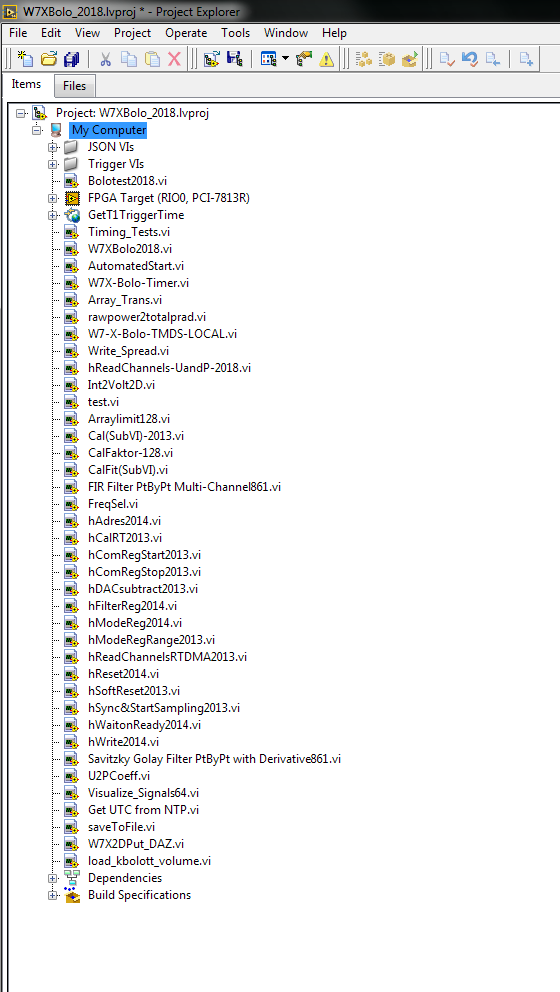
\includegraphics[height=0.8\textheight]{figures/content/project.png}%
          \caption{\tiny%
                   full software project with all dependencies; FPGA target %
                   with current build of executable and bit file, untouched %
                   (leave untouched!)}%
        \end{figure}%
      \column{0.45\textwidth}%
        \begin{block}{}%
          \begin{itemize}%
            \item{important files are `AutomatedStart.vi' \& `W7XBolo2018.vi'}%
            \item{latter is main VI in where %
                  calibration, acquisition and output are queued}%
            \item{'hReadChannels-UandP-2018.vi' does measurement/estimation, %
                  `test.vi' is a timing and reference test (disabled in the %
                  build)}%
            \item{`rawpower2totalprad.vi' calculates the final 
                  $P_{rad}$ after acquisition}%
          \end{itemize}%
        \end{block}%
      \end{columns}%
  \end{frame}%

  % new frame
  \begin{frame}%
    \only<1->{%
      \begin{figure}%
        \centering%
        \includegraphics[width=0.9\textwidth]%
          {figures/content/front_panel_daq_settings.png}%
        \caption{\tiny%
                 front panel: data acquisition and range settings for %
                 the voltage boundaries of the controller, e.g. %
                 turn/dial or file import of individual/global bits}%
      \end{figure}%
    }%
    \begin{block}{}
        \begin{itemize}
          \only<1>{%
            \item{time of acq. defined in seconds (divide by sampling rate in %
                  ms yields number of samples)}%
            \item{comparison of predicted DAQ duration and actual time passed %
                  acquiring samples (performance)}%
          }%
          \only<2>{%
            \item{switch between global (all channels the same), individual %
                  bit settings for DAC ranges}%
            \item{switch for input or file loaded settings of DAC ranges; %
                  individual input settings located in bottom `Test' tab}%
          }%
          \only<3>{%
            \item{trigger and current epoch time displayed at top of VI}%
            \item{countdown to start of data acquisition}%
          }%
        \end{itemize}
    \end{block}
  \end{frame}%

  % new frame
  \begin{frame}
    \begin{figure}
      \centering
      \includegraphics[height=0.8\textheight]%
        {figures/content/blockdiagramm_import_and_files.png}%
      \caption{block diagram 'W7XBolo2018.vi': of previous front panel parts %
        (top - timing, middle top - geometric factors import/input, %
        middle bottom - channel selection, %
        bottom - DAC range settings)}
    \end{figure}
  \end{frame}

  % frame
  \begin{frame}
    \only<1->{%
      \begin{figure}%
        \centering%
        \includegraphics[width=0.9\textwidth]%
          {figures/content/front_panel_trigger_settings.png}%
        \caption{\tiny%
                 front panel: trigger source settings and timings; pre-start %
                 time before T0 (60s fixed after hardware trigger)}%
      \end{figure}%
    }%
    \begin{block}{}
        \begin{itemize}
          \item{time of acq. defined in seconds (divide by sampling rate in %
                ms yields number of samples)}%
          \item{comparison of predicted DAQ duration and actual time passed %
                acquiring samples (performance)}%
        \end{itemize}
    \end{block}
  \end{frame}

  % frame
  \begin{frame}
    \begin{figure}%
      \centering%
      \includegraphics[width=0.9\textwidth]%
        {figures/content/front_panel_scanid_error.png}%
      \caption{\tiny%
               front panel: error top panel %
               (first place to look at if something goes wrong/seems off) %
               `ScanID read/write error' refers to the stashed sample number %
               on the FPGA target}%
    \end{figure}%
  \end{frame}

  % frame
  \begin{frame}
    \begin{columns}
      \column{0.6\textwidth}
        \begin{figure}%
          \centering%
          \includegraphics[width=0.9\textwidth]%
            {figures/content/front_panel_realtime_prad.png}%
          \caption{\tiny%
                   front panel: `Test' tab; various DAC range import and %
                   and load settings; channel selection settings for %
                   $P_{rad}$ estimation; array debugging and error codes}%
        \end{figure}%
      \column{0.4\textwidth}
        \begin{block}{}
          \begin{itemize}
            \only<1>{%
              \item{top: switches on what to import for DAC range/channel %
                    selection}
              \item{below: sampling and frequency settings for voltage %
                    output of $P_{rad}$ estimate, plus scaling voltage %
                    @ 10\,MW}
              \item{bottom: debugging for arrays of imports/input}
            }
          \end{itemize}
        \end{block}
    \end{columns}
  \end{frame}

  % frame
  \begin{frame}
    \begin{figure}
      \centering
      \includegraphics[width=0.8\textwidth]%
        {figures/content/blockdiagramm_channelsetup.png}%
      \caption{\tiny%
               block diagram 'W7XBolo2018.vi': flat sequence of DAQ %
               `hReadChannels-UandP-2018.vi' with local variables inputs; %
               bottom: channel set up for voltage and sampling on analog; %
               right, outside: end of analog sampling and %
               `rawpower2totalprad.vi', where the channel power is used %
               to calculate a `full' $P_{rad}$}%
    \end{figure}
  \end{frame}

  % frame
  \begin{frame}
    \begin{figure}%
      \centering%
      \includegraphics[width=0.9\textwidth]%
        {figures/content/front_panel_statuspanel.png}%
      \caption{\tiny%
               front panel: 'Status' panel tab; if calibration or %
               reference values are off, this shows the channel status %
               accordingly}%
    \end{figure}%
  \end{frame}

  % frame
  \begin{frame}
      \begin{figure}%
        \centering%
        \includegraphics[width=0.9\textwidth]%
          {figures/content/uandp_blockdiagramm_raw2power.png}%
        \caption{\tiny%
                 block diagram 'hReadChannels-UandP-2018.vi': %
                 conversion from raw voltage signal of channel and sample to %
                 power; bottom right: input for estimation routine and FIFO %
                 shifting}%
      \end{figure}%
  \end{frame}

  % frame
  \begin{frame}
      \begin{figure}%
        \centering%
        \only<1>{%
          \includegraphics[width=0.9\textwidth]%
            {figures/content/uandp_blockdiagramm_estimation_less10.png}%
          \caption{\tiny%
                   block diagram 'hReadChannels-UandP-2018.vi': %
                   first part of estimation - before 10th sample, filling up %
                   averaging FIFO array}%
        }%
        \only<2>{%
          \includegraphics[width=0.9\textwidth]%
            {figures/content/uandp_blockdiagramm_estimation_greater10.png}%
          \caption{\tiny%
                   block diagram 'hReadChannels-UandP-2018.vi': %
                   after 10th sample, averaging with geometry factors and %
                   scaling; then FIFO push the first sample out for new one %
                   (far right) and writing to the referenced properties for %
                   the top level `W7XBolo2018.vi'}%
        }%
      \end{figure}%
  \end{frame}

  % frame
  \begin{frame}
      \begin{figure}%
        \centering%
        \includegraphics[width=0.9\textwidth]%
          {figures/content/channels2prad_blockdiagram.png}%
        \caption{\tiny%
                 block diagram 'rawpower2totalprad.vi': %
                 processing routine calculating the `full' $P_{rad}$ after %
                 acquisition has finished, hence for all channels and %
                 samples the same calculation as in the previous subVI}%
      \end{figure}%
  \end{frame}

  % frame
  \begin{frame}
    \only<1>{%
      \begin{exampleblock}{Pros:}
        \begin{itemize}
          \item{performance good for channel selection of up to $\sim$10}
          \item{acquisition times for one sample actually improved due to %
                some touch ups compared to old version}
          \item{technicality of imports, inputs and loading has been proven %
                to not fail in previous (trigger-) tests}%
          \item{stash of local files to load configuration, reproducibility}
          \item{calculation of estimate $P_{rad}$ seems fine, tests to be %
                made with comparison signal (manual/virtual)}
        \end{itemize}
      \end{exampleblock}
    }
    \only<2>{%
      \begin{alertblock}{Cons:}
        \begin{itemize}
          \item{critical bug/feature in LabView's abort/stop function that %
                does not clear FPGA targets local memory, hence e.g. samples %
                acquired is stuck on a specific value}
          \item{hence, no proper measurement is possible directly after a %
                failed software deployment/execution}
          \item{calculation inside `rawpower2totalprad.vi' seem to be off by %
                some orders of magnitude $10^{x}$ to no apparent reason %
                (exactly the same calculation process as in `hReadChannels-UandP-2018.vi')}
          \item{?! to be proven: upload to archive broken ?!}
        \end{itemize}
      \end{alertblock}
    }
    \only<3>{%
      \begin{block}{TODO:}
        \begin{itemize}
          \item{fix upload cycle and add the current configurations to it in %
                the form of a JSON, add estimation time line to archive}
          \item{proof of calculations and estimation}
          \item{find possible fix for memory cache, local flashing routine of %
                FPGA target in the start up phase of VI maybe}
          \item{fix full $P_{rad}$ routine}
        \end{itemize}
      \end{block}
    }
  \end{frame}

  % \begin{frame}{Bibliography}
  %   \backgroundlogo
    % BIBLIOGRAPHY
    % \only<1>{\footnotesize%
    %   \begin{thebibliography}{}%
    %     \bibitem{Zhang2010} "Design Criteria of the Bolometer diagnostic %
    %                         for steady-state operation of the W7-X %
    %                         stellarator"; %
    %                         Zhang, D. et al.; %
    %                         Review of Scientific Instruments, %
    %                         Jan 1st, 2010; DOI:10.1063/1.3483194
    %   \end{thebibliography}%
    % }
  % \end{frame}%

  % EMPTY FRAME
  % \begin{frame}{}
  %   \backgroundlogo
  % \end{frame}

  % BACKUP
  \appendix
  \backupbegin

  \begin{frame}{Appendix}%
    \begin{figure}%
      \centering%
      \only<1>{%
        \includegraphics[width=0.9\textwidth]%
          {figures/content/channels2prad_blockdiagramm_new_power_routine.png}%
      }%
      \only<2>{%
        \includegraphics[width=0.9\textwidth]%
          {figures/content/power_factors_blockdiagramm.png}%
      }
    \end{figure}%
  \end{frame}

  % BACKUPEND
  \backupend

\end{document}